%=============================================================================%
% Preamble
%=============================================================================%
% Libraries

\documentclass[xcolor=table]{beamer}
%\usepackage{beamerthemeshadow}
\usepackage{helvet}
\usepackage[]{graphicx}
\usepackage{array}
\usepackage{color}
\definecolor{dkgreen}{rgb}{0,0.6,0}
\definecolor{gray}{rgb}{0.5,0.5,0.5}
\definecolor{mauve}{rgb}{0.58,0,0.82}
\definecolor{deepblue}{rgb}{0,0,0.5}
\definecolor{deepred}{rgb}{0.6,0,0}
\definecolor{deepgreen}{rgb}{0,0.5,0}
\definecolor{lightgray}{rgb}{0.92,0.92,0.92}
\usepackage{listings} % to insert code
\usepackage{textpos} % textblock
\usepackage{hyperref}
\hypersetup{colorlinks=true, urlcolor=blue, linkcolor=black} 
% Listing set up
% bash
\lstdefinestyle{bash}{
language=bash,                     % the language of the code
basicstyle=\scriptsize\ttfamily,       % the size of the fonts that are used for the code
numbers=none,%left,                   % where to put the line-numbers
numberstyle=\tiny\color{gray},  % the style that is used for the line-numbers
stepnumber=1,                   % the step between two line-numbers. If it's 1, each line
                          % will be numbered
numbersep=5pt,                  % how far the line-numbers are from the code
backgroundcolor=\color{lightgray},  % choose the background color. You must add \usepackage{color}
showspaces=false,               % show spaces adding particular underscores
showstringspaces=false,         % underline spaces within strings
showtabs=false,                 % show tabs within strings adding particular underscores
frame=lines,%single,                   % adds a frame around the code
rulecolor=\color{black},        % if not set, the frame-color may be changed on line-breaks within not-black text (e.g. commens (green here))
tabsize=2,                      % sets default tabsize to 2 spaces
captionpos=b,                   % sets the caption-position to bottom
breaklines=true,                % sets automatic line breaking
breakatwhitespace=false,        % sets if automatic breaks should only happen at whitespace
title=\lstname,                 % show the filename of files included with \lstinputlisting;
                          % also try caption instead of title
keywordstyle=\color{blue},      % keyword style
commentstyle=\color{dkgreen},   % comment style
stringstyle=\color{mauve},      % string literal style
escapeinside={\%*}{*)},         % if you want to add a comment within your code
morekeywords={}            % if you want to add more keywords to the set
}

\lstdefinestyle{python}{
language=python,
formfeed=\newpage,
basicstyle=\scriptsize\ttfamily,
commentstyle=\color{deepgreen},%\color{gray},
numbers=left,
numberstyle=\tiny\color{gray},
stepnumber=1,
numbersep=5pt,
backgroundcolor=\color{lightgray},%\color{white},
showspaces=false,
showstringspaces=false,
showtabs=false,
frame=lines,
tabsize=4,
captionpos=b,
breaklines=true,
breakatwhitespace=false,
title=\lstname,
escapeinside={},
keywordstyle=\color{deepblue},
emphstyle=\color{deepred},
stringstyle=\color{deepgreen}
%morekeywords={models, lambda, forms}
}

\graphicspath{ {../img/} }

\begin{document}
\title{Python for Scientific Research}   
\author{Bram Kuijper}
\institute[]{University of Exeter, Penryn Campus, UK}
\titlegraphic{
\hfill

\includegraphics[width=\textwidth, keepaspectratio]{logo.jpg}}

\frame{\titlepage} 
\begin{frame}{Acknowledgements}
\begin{itemize}\addtolength{\itemsep}{\baselineskip}
    \item This course is funded by UExeter's Institute for Data Science and Artificial Intelligence: \href{https://www.exeter.ac.uk/idsai/}{IDSAI}
	\item Big thanks to \href{https://emps.exeter.ac.uk/mathematics/staff/jjv207}{JJ Valletta} as he has developed these lectures 
    \item Big thanks to \href{http://emps.exeter.ac.uk/mathematics/staff/dp457}{Deepak Kumar Panda} for helping out this afternoon 
\end{itemize}
\vfill

\includegraphics[width=\textwidth, keepaspectratio]{logo.jpg}

\end{frame}

\frame{
    \frametitle{Course Schedule} 
    \begin{itemize}
        \item Tuesday Feb 4: The basics of programming in Python
            \begin{itemize}
                \item how to run Python code
                \item data types
                \item flow control
                \item functions and modules
            \end{itemize}
            \pause
        \item Tuesday Feb 11: Applying Python to simplify your life
            \begin{itemize}
                \item text manipulation and regular expressions
                \item working with files and streams
                \item number crunching with \texttt{numpy} and \texttt{scipy}
            \end{itemize}
            \pause
        \item Tuesday Feb 25: Advanced subjects
            \begin{itemize}
                \item working with data using \texttt{pandas}
                \item making graphs using \texttt{matplotlib}
                \item data visualisation with \texttt{seaborn}
            \end{itemize}
    \end{itemize}
}

\frame{
    \frametitle{Schedule Tue Feb 4} 
% TODO  work on refining schedule
    \begin{itemize}
        \item Morning session, 0900 - 1100 DDM IT 3.037
    \begin{itemize}
        \item 0900 - 0930: How to run Python
        \item 0930 - 1000: Data types
        \item 1000 - 1010: Break
        \item 1010 - 1100: Data types practical
    \end{itemize}
        \item Afternoon session, 1300 - 1600 DDM IT 1.033
    \begin{itemize}
        \item 1300 - 1300: Flow control
        \item 1330 - 1400: Flow control practical
        \item 1400 - 1410: Break
        \item 1410 - 1430: Flow control practical continued 
        \item 1410 - 1500: Functions practical
        \item 1410 - 1500: Functions practical
    \end{itemize}
    \end{itemize}
}

\frame{\frametitle{Some important websites}
\begin{itemize}
    \item Course website: \url{https://exeter-data-analytics.github.io}
    \item Python documentation: \url{https://docs.python.org}
\end{itemize}
}

\frame{\frametitle{What is Python?}
\begin{itemize}
    \item A scripted, high-level programming language created by Guido Van Rossum and named after Monty Python's flying circus
\begin{center}
    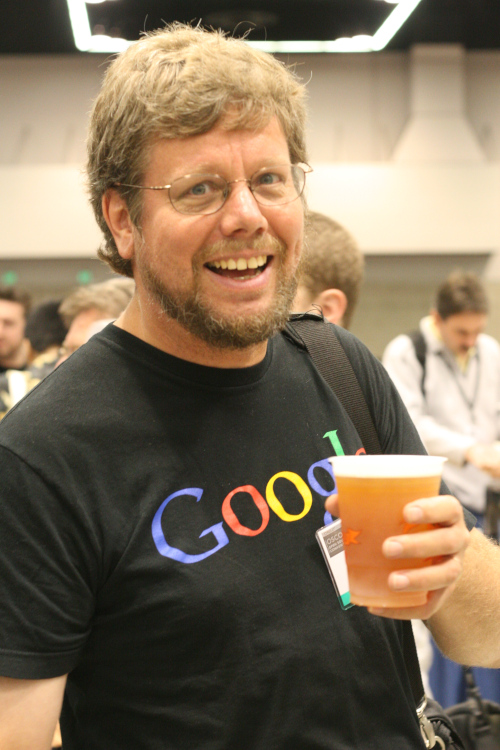
\includegraphics[width = 20mm]{GuidoVanRossumSmall.jpg}
    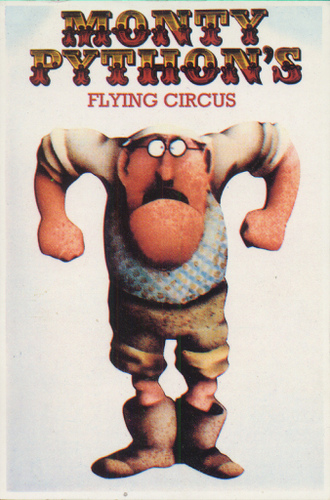
\includegraphics[width = 20mm]{MontyPython.jpg}
\end{center}
    \pause
    \item easy-to-use, highly standardized and with an emphasis on readability of code
\end{itemize}
}


\frame{\frametitle{Why use Python?}
The TIOBE index is a measure of the popularity of programming languages:
    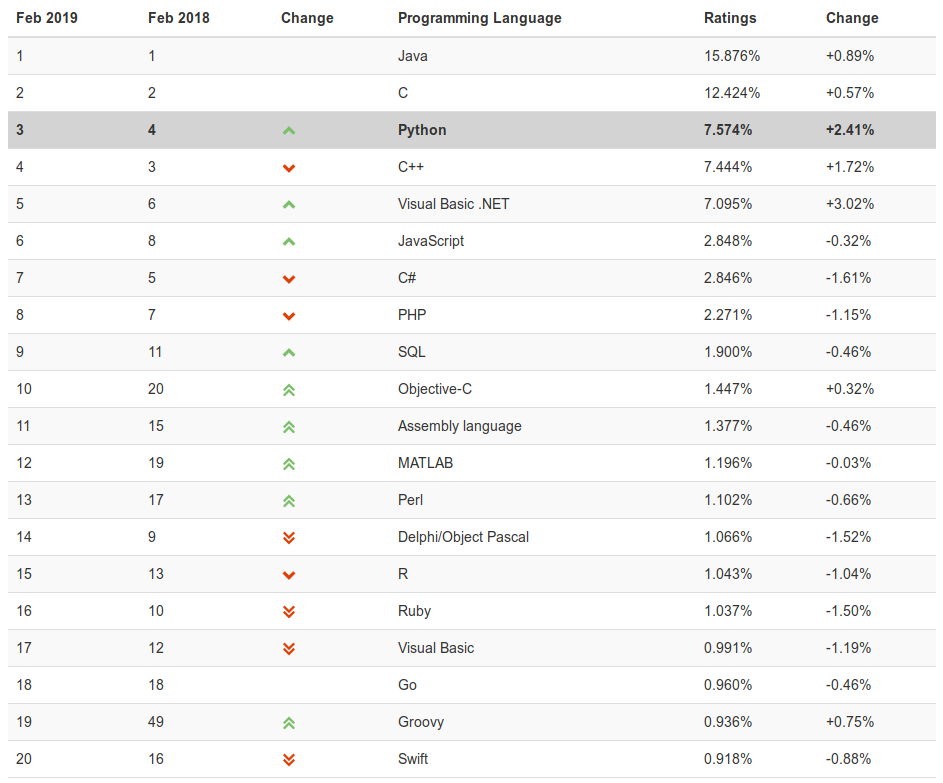
\includegraphics[width = 10cm]{TiobeIndex.png}
}

\begin{frame}{Why Python?}
%. Here are some reasons for its popularity:

\begin{itemize}\addtolength{\itemsep}{0.5\baselineskip}
	\item<1-> It is free! No licence costs
	\item<2-> Runs on many platforms (Mac, Windows, Linux)
	\item<3-> Because of its ease of programming, Python minimises development effort
	\item<4-> A huge number of \href{https://pypi.python.org/pypi}{libraries}, written by an active \href{https://www.python.org/community/}{community}  
	\item<5-> Python can ``glue" together functions written in C/C++ and Fortran to speed things up (we can also call R and MATLAB functions)
	\item<6-> Compared to other high-level scientific languages such as MATLAB and R, Python offers a much wider range of additional functionality (e.g \href{https://www.djangoproject.com/}{web} and \href{https://wiki.python.org/moin/TkInter}{GUI} development) %hence the nickname ``the swiss army knife" of programming languages. 
\end{itemize}

\end{frame}

%=============================================================================%
%=============================================================================%
\begin{frame}{Horses for courses}

\begin{itemize}\addtolength{\itemsep}{0.5\baselineskip}
        \item<1-> Python is becoming the \emph{de facto} standard for exploratory and interactive scientific research\\
	\item[]<1-> \textbf{BUT}
	\item<2-> Python is no programming silver bullet
	\item<3-> Your application will dictate the tool (and a mixture of more than one language is ok). For example:\\
	\begin{itemize}\addtolength{\itemsep}{0.8\baselineskip}
		\item<4-> MATLAB excels at interfacing with hardware, e.g generating \href{https://uk.mathworks.com/products/hdl-coder.html}{hardware description language (HDL) code} to configure an integrated circuit board or connecting to a \href{https://uk.mathworks.com/products/daq.html}{data acquisition card}
		\item<5-> R is great for data wrangling and visualisation, and statistical modelling
        \item<6-> C achieves the fastest runtimes, at the expense of a long development time
	\end{itemize}
\end{itemize}

\end{frame}


\begin{frame}{Why do \textit{you} want to learn Python?}
    Some reasons:
    \pause
    \begin{itemize}
        \item Python has a simple syntax and is widely used; ideal language for beginners
            \pause
        \item Development time is much quicker than for compiled languages like C or Java
            \pause
        \item Broad uptake: Python (and R) have replaced Perl as the key programming language in Bioinformatics
            \pause
        \item major GIS applications like ArcGIS use Python as their main scripting language
        \item Language of choice for machine learning (PyTorch, scikit, TensorFlow)
            \pause
    \end{itemize}
\end{frame}

\frame{\frametitle{Python version 2 vs 3}
    \begin{itemize}
        \item Many systems (e.g., Mac OS X) still use Python 2 as the default
        \item Python 3 differs in \href{https://sebastianraschka.com/Articles/2014\_python\_2\_3\_key\_diff.html}{various ways} from Python 2
        \item Often, Python 3 code cannot be run using a Python 2 interpreter and vice versa
        \item Python 2 is a legacy version and will ultimately be replaced by Python 3
        \item \textbf{Current course will focus on Python 3}
    \end{itemize}
}

\frame{\frametitle{Different Python distributions}
Various distributions of Python available:
    \begin{itemize}
            \pause
        \item Official version from \href{https://python.org}{python.org} 
            \begin{itemize}
                \item Caveat: libraries and other tools need to be installed separately via \texttt{pip} (Python's package manager)
        \end{itemize}
            \pause
        \item \href{https://www.enthought.com/product/canopy/}{Enthought Canopy}: Python, libraries \& tools in single installer
            \pause
        \item \href{https://www.anaconda.com/distribution/}{Anaconda}: Python, libraries \& tools in single installer: \textbf{used in this course}
            \begin{center}

\includegraphics[width=0.3\textwidth]{AnacondaLogo.png}
            \end{center}
            \pause
    \end{itemize}
}


\begin{frame}[fragile]
\frametitle{Executing Python code: Spyder IDE}
    \begin{itemize}
        \item Windows: Start Menu $>$ Anaconda3 $>$ Spyder
            \pause
        \item Mac: Applications $>$ Spyder
    \end{itemize}
\end{frame}

\begin{frame}[fragile]
\frametitle{Executing Python code: Spyder IDE}
\begin{itemize}\addtolength{\itemsep}{.7\baselineskip}
	\item Spyder is an integrated development environment (IDE) for scientific computing, akin to \href{https://www.rstudio.com/}{RStudio} and \href{https://uk.mathworks.com/products/matlab.html}{MATLAB} 
	\item One place to write, execute and debug code, and explore variables
\end{itemize}

\begin{center}
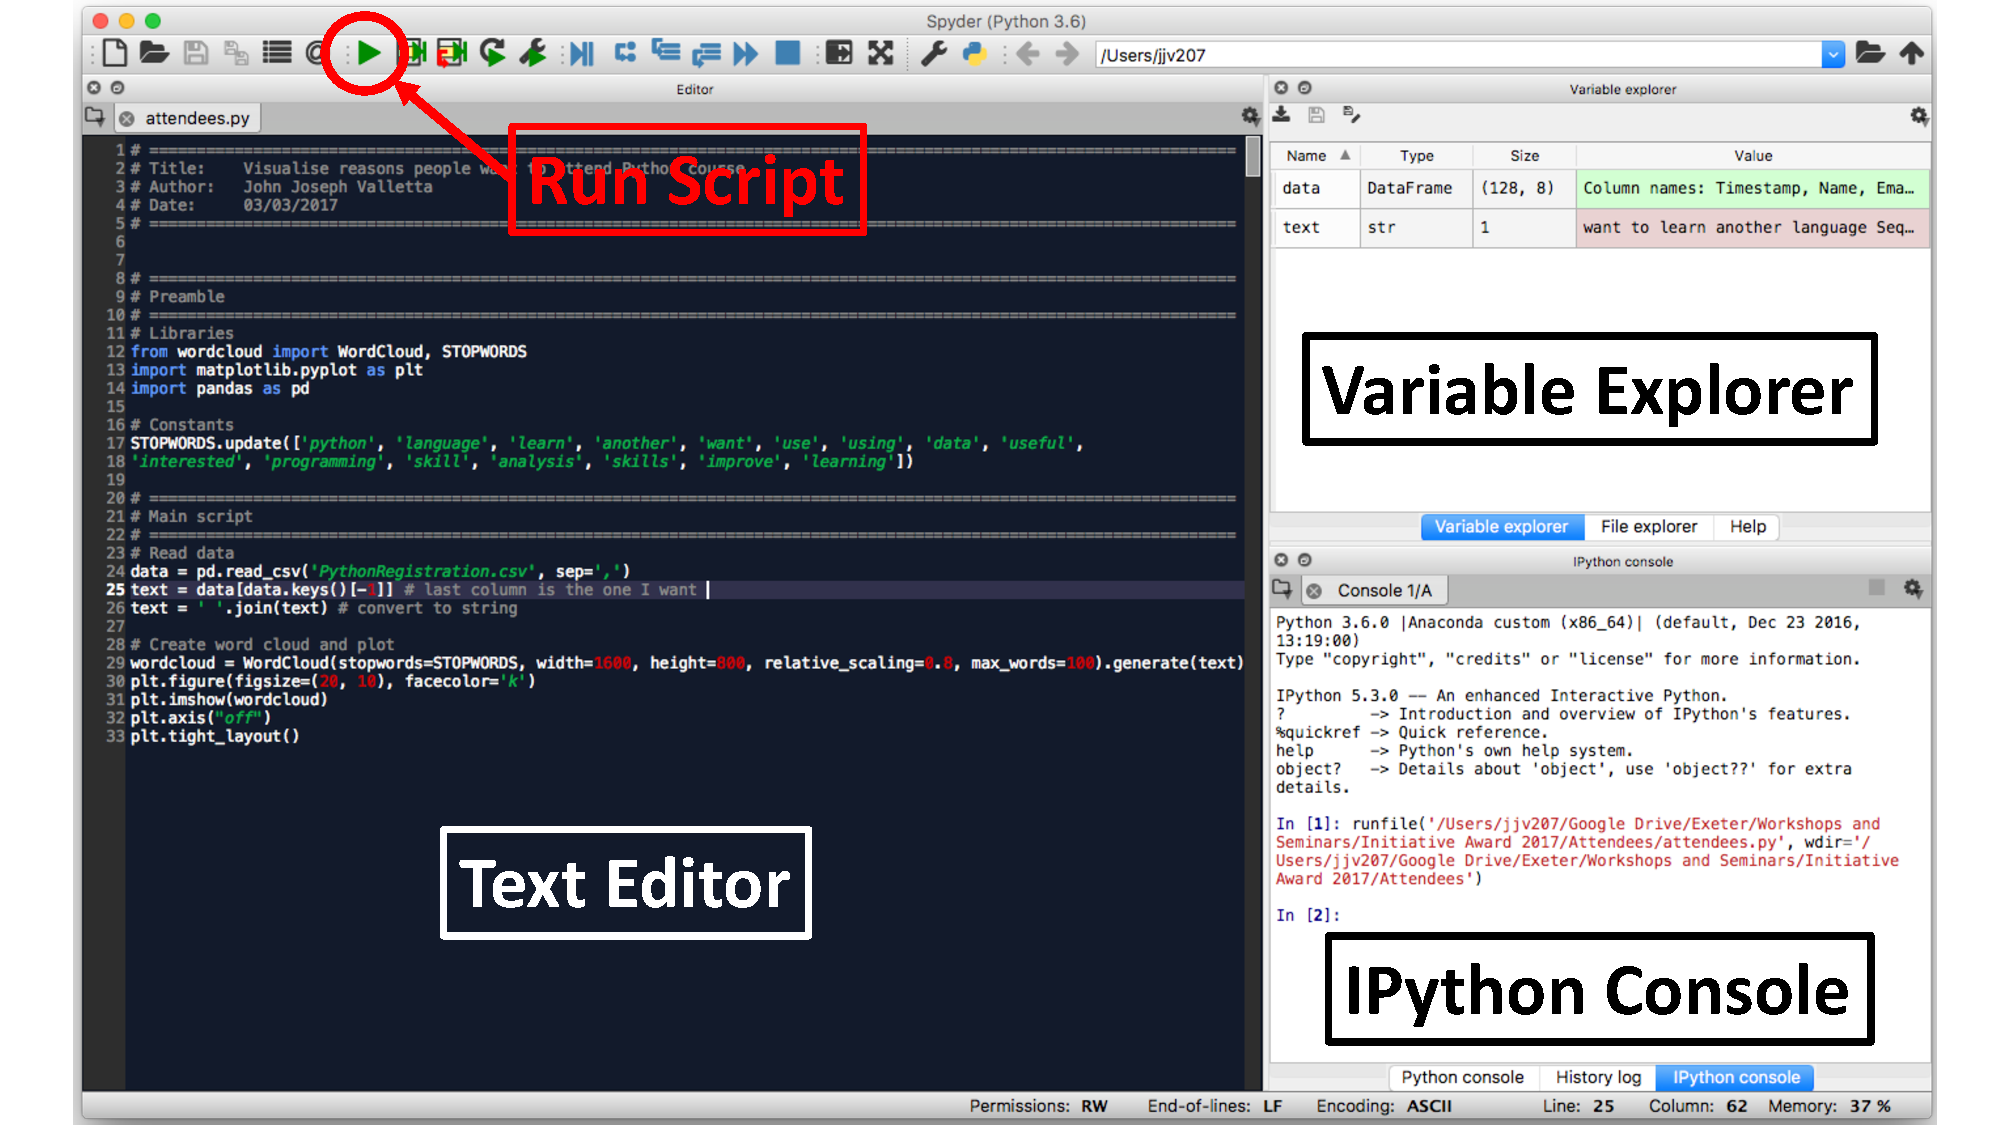
\includegraphics[width=0.8\textwidth]{spyder_annotated.pdf}
\end{center}
\end{frame}

\begin{frame}[fragile]
\frametitle{Running standalone Python scripts without the IDE - I}
Being able to run Python scripts without the Spyder IDE is particularly important when running scripts on computing clusters. 

    
\begin{itemize}
    \item Windows: don't bother, use the Spyder IDE
        \pause
    \item Mac/Linux: 
        \begin{itemize}
            \item Write your code in a plain text file, say \texttt{my\_script.py}
                \pause
            \item In a terminal, run:
\begin{lstlisting}[style=bash]
python3 my_script.py
\end{lstlisting}
\end{itemize}
\end{itemize}

\end{frame}


\begin{frame}[fragile]
\frametitle{Running standalone Python scripts without the IDE - II}
By adding a so-called `shebang' to the top of a Python script, one 
can run scripts as a standalone programme on Mac / Linux \vspace{3pt}
   \pause 
\begin{itemize}\addtolength{\itemsep}{0.05\baselineskip}
    \item Add a shebang \texttt{\#!/usr/bin/env python3}, to the first line of the python script file, here called \texttt{my\_script.py}:
\begin{lstlisting}[style=python]
#!/usr/bin/env python3

print("This Python script prints something.")
...
\end{lstlisting}
    \pause 
    \item Close the file and make it executable by typing in a terminal
\begin{lstlisting}[style=bash]
chmod +x my_script.py
\end{lstlisting}
    \pause 
    \item Run the script by typing in a terminal
\begin{lstlisting}[style=bash]
./my_script.py
This Python script prints something.
\end{lstlisting}
\end{itemize}

\end{frame}

\end{document}

